\chapter{Version control with Git}
\label{chap:git}

\section{What is Version Control?}

Version control, also known as revision control or source control, is 
the management and tracking of changes to documents, computer programs, 
large web sites, and other collections of information in an automated 
way.

Any project (collections of files in directories) under version control 
has changes and additions/deletions to its files and directories 
recorded and archived over time so that you can recall specific 
versions later. With version control of biological computing projects, 
you can:

 \begin{compactitem}\itemsep10pt{}
 
		\item record of all changes made to a set of files and directories, 
		including text (usually ASCII) data files, so that you can access 
		any previous version of the files

    \item branch (and merge) new projects

		\item ``roll back'' data, code, documents that are in plain text 
		format (other file formats can also be versioned; see section on 
		binary files below). 
	
	\end{compactitem}
 
Note also that version control (usually git) is in fact the technology 
embedded in the versioning of various word processor and  
spreadsheet applications (e.g., Google Docs, Sheets, Overleaf). 

\begin{figure} \centering
  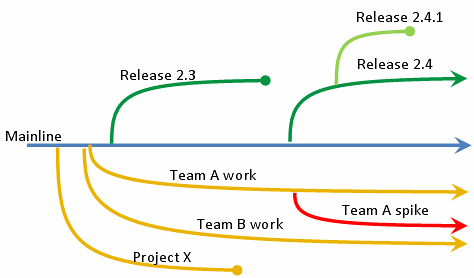
\includegraphics[width=.5\textwidth]{VC.png}
  \caption{A general idea of how version control works.}
\end{figure}

\section{Why Version Control?}

{\centering  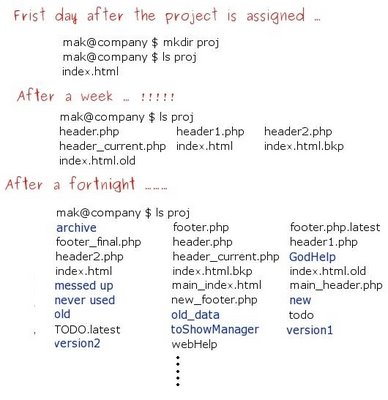
\includegraphics[width=.5\textwidth]{cvs.png}\\
  \tt 
maktoons.blogspot.com/2009/06/if-dont-use-version-control-system.html}
 
 Or here's another one: \url{http://www.phdcomics.com/comics/archive/phd101212s.gif} 
  
\section{git}

We will use git, developed by Linus Torvalds, the ``Linu'' in Linux. In 
git each user stores a complete local copy of the project, including the 
history and all versions. So you do not rely as much on a centralized 
(remote) server. We will use bitbucket.org -- it gives you unlimited 
free private repositories if you register with an academic email! 
First, install and configure {\tt git}:

\begin{lstlisting} 
$ sudo apt-get install git
$ git config --global user.name "Your Name"
$ git config --global user.email "your.login@imperial.ac.uk"
$ git config --list
\end{lstlisting}

\section{Your first repository}

Time to bring your {\tt CMEECourseWork} under version control:

\begin{lstlisting} 
$ cd CMEECourseWork
$ git init
$ echo "My CMEE 2016-17 Coursework Repository" > README.txt
$ git config --list
$ ls -al
$ git add README.txt #Staging
$ git status
$ git commit -m "Added README file." #you can use -am too
$ git status #what does it say now?
$ git add -A
$ git status
\end{lstlisting} 

Nothing has been sent to a remote server yet (see section 
\ref{ssec:git_comds})! So let's go to your git service (bitbucket or 
github) and setup:

 \begin{compactitem}[$\quad\star$]\itemsep4pt
	\item Login to your bitbucket or github account
	\item \sloppy Set up your {\tt ssh} based access 
	
	bitbucket:
	\url{https://confluence.atlassian.com/bitbucket/set-up-ssh-for-git-728138079.html} 
	
	github: \url{https://help.github.com/articles/connecting-to-github-with-ssh}
  
  \item Then create repository there with name {\tt CMEECourseWork}
	
	\item \sloppy Then grab the repository url and use {\tt git remote add origin 
	https...} 
	
	bitbucket:  \url 
	{https://confluence.atlassian.com/bitbucket/set-up-a-repository-877174034.html}
	
	github: \url{https://help.github.com/articles/adding-an-existing-project-to-github-using-the-command-line/}
	
 \end{compactitem}
  	  
You are done. Now let's learn to use git! 

\section{{\tt git} commands}
  
Here are some basic git commands:
 
\begin{tabular}{p{.3\textwidth} p{.7\textwidth}} 
	{\tt git init} & Initialize a new repository\\
	{\tt git clone} & Download a repository from a remote server\\
	{\tt git status} & Show the current status\\
	{\tt git diff} & Show differences between commits\\
	{\tt git blame} & Blame somebody for the changes!\\
	{\tt git log} & Show commit history\\
	{\tt git commit} & Commit changes to current branch\\
	{\tt git branch} & Show branches\\
	{\tt git branch name} & Create new branch\\
	{\tt git checkout name} & Switch to a different commit/branch\\
	{\tt git pull} & Upload from remote repository\\
	{\tt git push} & Send changes to remote repository\\
\end{tabular}

\subsection{{\tt git} command structure}
\label{ssec:git_comds}
Here is a graphical outline of the git command structure. Note that 
only when you {\tt push} or  {\tt fetch} do you need an internet 
connection, as before that you are only archiving in a local (hidden) 
repository. 
 
  \begin{center}
		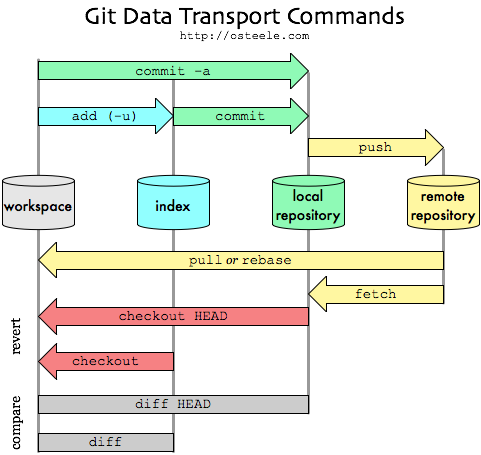
\includegraphics[width=.6\textwidth]{git.png}
	\end{center}

Keep in mind, the main mantra is, ``commit often, comment always''!

  \begin{center}
		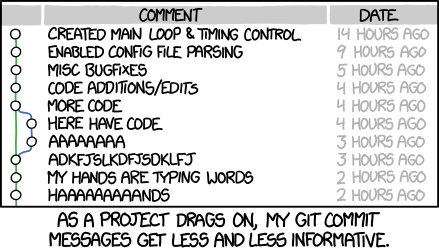
\includegraphics[width=.6\textwidth]{git_xkcd.png}
	\end{center}
	 
\section{Ignoring Files}

You will have some files you don't want to track (log files, temporary 
files, executables, etc). You can ignore entire classes of files with 
{\tt .gitignore} (be in your {\tt CMEECourseWork}!):

\begin{lstlisting}
$ echo -e "*~ \n*.tmp" > .gitignore

$ cat .gitignore
*~
*.tmp

$ git add .gitignore

$ touch temporary.tmp

$ git add *
The following paths are ignored by one of your .gitignore 
files:
temporary.tmp
Use -f if you really want to add them.
fatal: no files added
\end{lstlisting}

You can also create a global gitignore file that lists rules for files 
to be ignored in every Git repository on your computer:  
\url{https://help.github.com/articles/ignoring-files/} 

\subsection{Dealing with binary files}

A binary file is computer-readable but not human-readable, that 
is, it cannot be read by opening them in a text viewer. Examples of 
binary files include compiled executables, zip files, images, word 
documents  and videos. In contrast, text files are stored in a form (usually ASCII) 
that is human-readable by opening in a suitable text reader (e.g., 
geany, gedit). Without some git extensions and configurations (coming up 
next), binary files cannot be properly version-controlled because each version of
the entire file is saved {\it as is} in a hidden directory in the repository ({\tt .git}).

However, with some more effort, git can be made to work for binary formats like *.docx or image formats 
such as *.jpeg, but it is harder to compare versions; have a look at 
\url{https://git-scm.com/docs/gitattributes} and 
\url{https://git-scm.com/book/en/v2/Customizing-Git-Git-Attributes}\footnote{There you will find the following phrase: ``...one of the most annoying problems known to humanity: version-controlling Microsoft Word documents.'' . LOL!} 

Also see: \url{https://opensource.com/life/16/8/how-manage-binary-blobs-git-part-7}
  
\subsection{Dealing with large files}

As such, git was designed for version control of workflows and software 
projects, {\it not} large files (say, >100mb) (which may be plain-text 
or binary). Binary files are particularly problematic because each version of
the file is saved {\it as is} in \texttt{.git}, when you have a large 
number of versions it means that there
are the same number of binary files in the hidden directory (for example
100 $\times$ >100mb files!). 

In this course at least, you should not try to keep large files 
(especially binary files under version control). You will run into this 
problem in the GIS week (where you will have to handle and store large 
raster image files) in particular \footnote{None of the computing weeks 
assessments will require you to use such large files anyway}. We 
suggest that you include files larger than some size in your 
{\tt .gitignore}.  For example, you can use the following bash command: 
\begin{lstlisting}
find . -size +100M | cat >> .gitignore	
\end{lstlisting}
The 100M means 100 mb -- you can reset it to whatever you want.  

You may also explore alternatives such as {\tt git-annex} 
(e.g., see \url{https://git-annex.branchable.com/}), and {\tt git-lfs} 
(e.g., see \url{https://www.atlassian.com/git/tutorials/git-lfs}).   

\section{Removing files}

To remove a file (i.e. stop version controlling it) use {\tt git rm}:

\begin{lstlisting} 
$ echo "Text in a file to remove" > FileToRem.txt

$ git add FileToRem.txt

$ git commit -am "added a new file that we'll remove later"
master 5df9e96 added a new file that we'll remove later
 1 files changed, 1 insertions(+), 0 deletions(-)
 create mode 100644 FileToRem.txt

$ git rm FileToRem.txt
rm 'FileToRem.txt'

$ git commit -am "removed the file"
master b9f0b1a removed the file
 1 files changed, 0 insertions(+), 1 deletions(-)
 delete mode 100644 FileToRem.txt
\end{lstlisting}
  
I typically just do all my stuff and then just use {\tt git add -A}  

\section{Accessing history of the repository}

To see particular changes introduced, read the repo's log :

\begin{lstlisting} 
$ git log
commit 08b5c1c78c8181d4606d37594681fdcfca3149ec
Author: Your Name <your.login@imperial.ac.uk>
Date:   Wed Oct 8 16:41:51 2014 -0500

    removed the file

commit 13f701775bce71998abe4dd1c48a4df8ed76c08b
Author: Your Name <your.login@imperial.ac.uk>
Date:   Wed Oct 5 16:41:16 2015 -0500

    added a new file that we'll remove later

commit a228dd3d5b1921ef18c5efd926ef11ca47306ed5
Author: Your Name <your.login@imperial.ac.uk>
Date:   Wed Oct 5 10:03:40 2015 -0500

    Added README file
\end{lstlisting}

For a more detailed version, add {\tt -p} at the end.
  
\section{Reverting to a previous version}

If things go horribly wrong with new changes, you can revert to the 
previous, ``pristine'' state:

\begin{lstlisting} 
$ git reset --hard
$ git commit -am "returned to previous state" #Note I used -am here
\end{lstlisting}

If instead you want to move back in time (temporarily), first find the 
``hash'' for the commit you want to revert to, and then check-out:

\begin{lstlisting} 
$ git status
# On branch master
nothing to commit (working directory clean)

$ git log
commit c797824c9acbc59767a3931473aa3c53b6834aae
Author: Your Name <your.login@imperial.ac.uk>
Date:   Wed Aug 22 16:59:02 2014 -0500
.
.
.

$ git checkout c79782
\end{lstlisting}

Now you can play around. However, if you commit changes, you create a 
``branch'' (git plays safe!). To go back to the future, type {\tt git 
checkout master}

\section{Branching}

Imagine you want to try something out, but you're not sure it will work 
well. For example, say you want to rewrite the Introduction of your 
paper, using a different angle, or you want to see whether switching to 
a library for a piece of code improves speed. What you then need is 
branching, which creates a project copy in which you can experiment:

\begin{lstlisting} 
$ git branch anexperiment

$ git branch
  anexperiment
* master

$ git checkout anexperiment 
Switched to branch 'anexperiment'

$ git branch 
* anexperiment
  master

$ echo "Do I like this better?" >> README.txt 

$ git commit -am "Testing experimental branch"
[anexperiment 9f17dc1] Testing experimental branch
 1 files changed, 2 insertions(+), 0 deletions(-)
\end{lstlisting}
 
If you decide to merge the new branch after modifying it:

\begin{lstlisting} 
$ git checkout master

$ git merge anexperiment
Updating 08b5c1c..9f17dc1
Fast-forward
 README.txt |    2 ++
 1 files changed, 2 insertions(+), 0 deletions(-)

$ cat README.txt 
My CMEE 2015-16 Coursework Repository
Do I like this better?
\end{lstlisting}

If there are no conflicts (i.e., some files that you changed also
changed in the master in the meantime), you are done, and you can
delete the branch:

\begin{lstlisting} 
$ git branch -d anexperiment
Deleted branch anexperiment (was 9f17dc1).
\end{lstlisting}

If instead you are not satisfied with the result, and you want to
abandon the branch:
\begin{lstlisting} 
$ git branch -D anexperiment
\end{lstlisting}

When you want to test something out, always branch! Reverting changes, 
especially in code, is typically painful. Merging can be tricky, 
especially if multiple people have simultaneously worked on a 
particular document. In the worst-case scenario, you may want to delete 
the local copy and re-clone the remote repository.

\begin{center}
	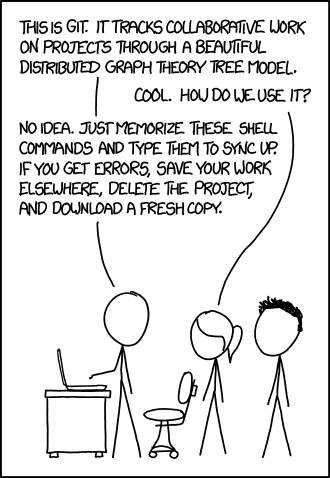
\includegraphics[width=.4\textwidth]{git_xkcd_1.png}
\end{center}
	
\section{Running git commands on a different directory}

Since {\tt git} version 1.8.5, you can run git directly on a 
different directory than the current one using absolute or relative 
paths. For example, using a relative path, you can do:
\begin{lstlisting}
git -C ../SomeDir/ status
\end{lstlisting}

\section{Running git commands on multiple repositories at once}
For git pulling in multiple subdirectories (each a separate 
repository):

\begin{lstlisting}
	$ find . -mindepth 1 -maxdepth 1 -type d -print -exec git -C {} pull \;
\end{lstlisting} 

Breaking down these commands one by one,

{\tt find .} searches the current directory\\
{\tt -type d} to find directories, not files\\
{\tt -mindepth 1} for setting min search depth to one sub-directory\\
{\tt -maxdepth 1} for setting max search depth to one sub-directory\\
{\tt -exec git -C \{\} pull $\textbackslash$ } runs a custom git command for every git repo found\\

\subsection[Practical]{Practicals}
  \begin{enumerate} \itemsep10pt
		\item The only practical submission for {\tt git} is the {\tt 
		.gitgnore} and overall git repository {\tt readme} file --- make 
		sure these in your coursework repository. 
		
		And of course, if you haven't gotten git with bitbucket 
		going, you won't be able to submit any of your practicals anyway!  
   
   \end{enumerate}


\section{Practical wrap-up}
   
  \begin{compactitem}

\item Invite me (s.pawar@imperial.ac.uk) to your {\tt CMEECourseWork} repository

\item The {\tt CMEEMasteRepo} will contain data and code files for 
upcoming practicals

\item You will clone {\tt CMEEMasteRepo} using {git clone 
git@bitbucket.org:mhasoba/cmee2015masterepo.git}

 \item You will thereafter {\tt git pull} {\tt CMEEMasteRepo}

\item You will {\tt git pull} inside {\tt CMEEMasteRepo} thereafter 
(always use {\tt git status} first)

\item {\tt cp} files from {\tt CMEEMasteRepo} to your {\tt 
CMEECourseWork} as and when needed --- don't work in the amster repo, 
as you will lose your work when I next update it! 

\end{compactitem}

\section{Readings \& Resources}

There is a wealth of information on {\tt git} out there - just google it!

\begin{compactitem}

\item Excellent book on Git: \url{http://git-scm.com/book}
\item Also, \url{https://www.atlassian.com/git/}
\item A git tutorial: \url{https://try.github.io}

\end{compactitem}
